\section*{BACKGROUND}
An effective interface to multiple robot programs is an important aspect to consider for a multi-robot applications simulation. The effort describes in this paper uses USARSim as a server allowing robot control programs (ROS)
to act as clients.

\subsection*{The USARSim Framework}


USARSim~\cite{CARPIN.LNAI.2006,WANG.WSC.2003} is a high-fidelity physics-based simulation system based on the industrial game engine Unreal Engine\footnote{http://www.unrealengine.com/}. USARSim was developed under a National Science Foundation grant to study Robot, Agent, Person Teams in Urban Search and Rescue~\cite{LEWIS.ICHC.2003}. Since Unreal Engine has been deployed for the development of networked multi-player 3D games, it solves many of the issues related to modeling, animation and rendering
of the virtual environment.

%Altogether, the Karma Physics engine~\cite{KarmEngine} and high-quality 3D rendering facilities of the Unreal game engine allow the creation of realistic simulation environments that provide the embodiment of a robotic system. Furthermore, USARSim comes with tools to develop objects and environments (Unreal Editor) and it is possible to control actors in the game through a TCP/IP socket API.

USARSimutilizes the Karma Physics engine~\cite{KarmEngine} and high-quality 3D rendering facilities of the Unreal game engine to create a realistic simulation environment that provides the embodiment of a robotic
system. The current release of USARSim consists of various environmental models, models of commercial and experimental robots, and sensor models. High fidelity at low cost is made possible by building the simulation on top of a game engine. By loading the most
difficult aspects of simulation to a high volume commercial platform which provides superior visual rendering and physical modeling, full effort can be devoted to the robotics-specific tasks of modeling platforms, control systems, sensors, interface tools and environments. These tasks are in turn, accelerated by the advanced editing and development tools integrated with the game engine leading to a virtuous spiral in which a wide range of platforms can be modeled with greater fidelity in short time.

USARSim was originally based upon simulated environments in the USAR domain.
Since then, USARSim has been used worldwide and more environments have been developed for different purposes. In addition to USAR, the simulator has been applied to the DARPA Urban Challenge (see Figure~\ref{3D_World-a}). Other environments such as the NIST campus (see Figure~\ref{3D_World-b}) and factories (see Figure~\ref{3D_World-c}) have been used to test the performance of algorithms in different efforts~\cite{WANG.HFES.2005,BALAGUER.IROS.2008,KOOTBALLY.ITEA.2010}.

\begin{figure}[t!]
\centering
\subfigure[ARDA.]{\label{3D_World-a}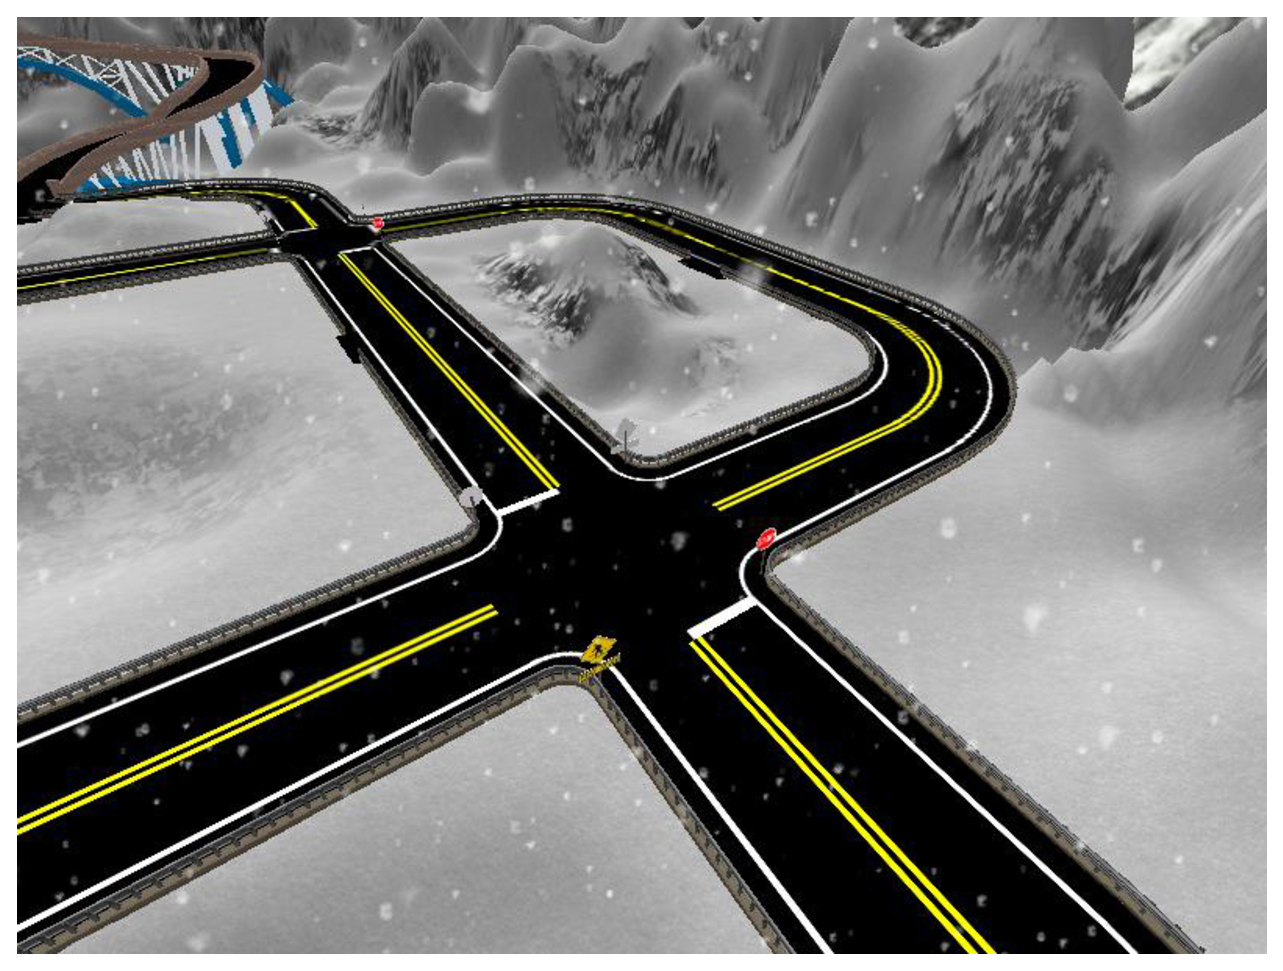
\psfig{file=Figures/Worlds/arda1.eps,width=4cm}}\qquad
\subfigure[NIST main
campus.]{\label{3D_World-b}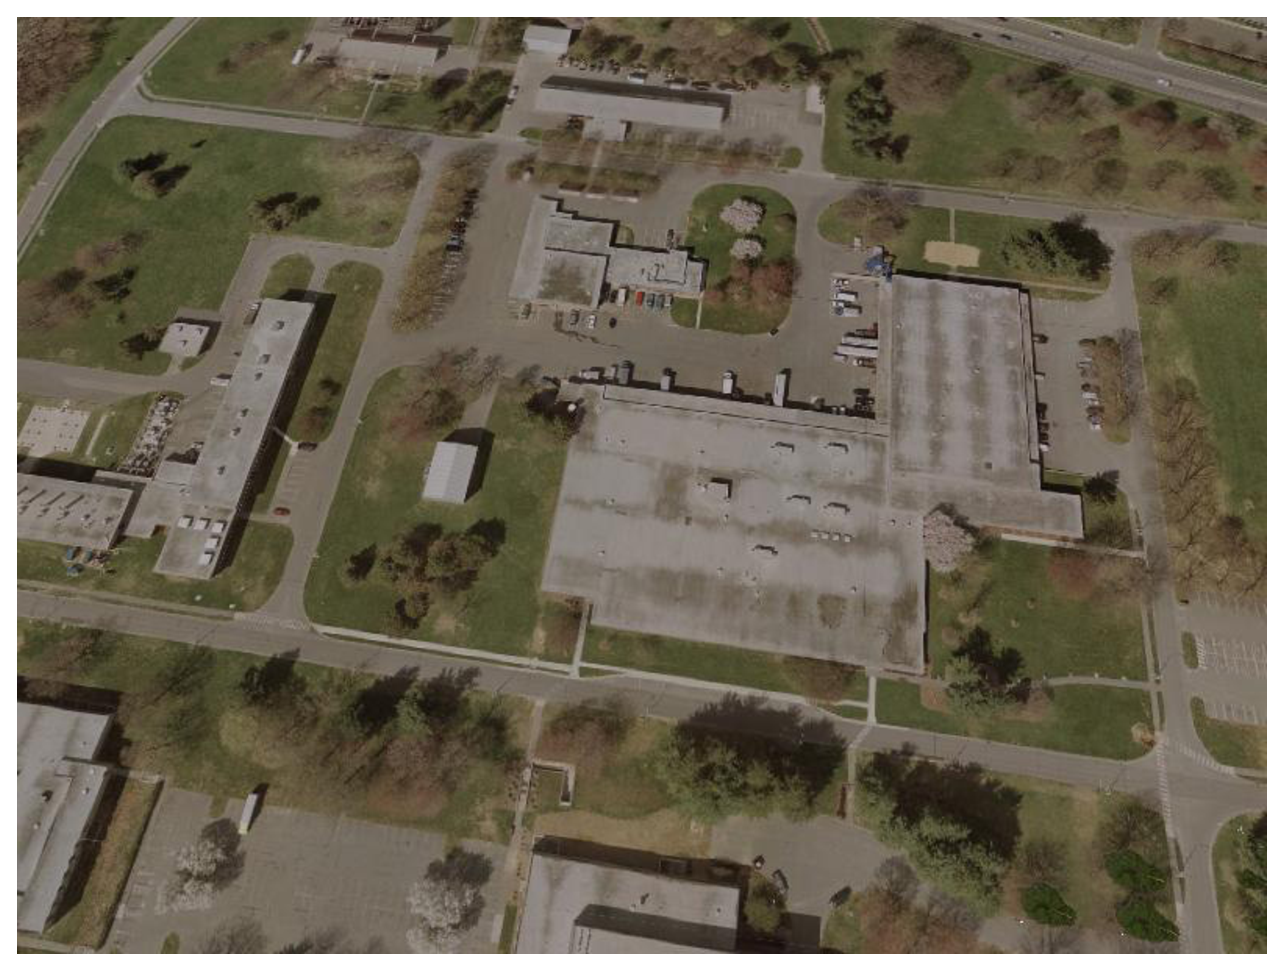
\psfig{file=Figures/Worlds/nist1.eps,width=4cm}}\qquad
\subfigure[Factory.]{\label{3D_World-c}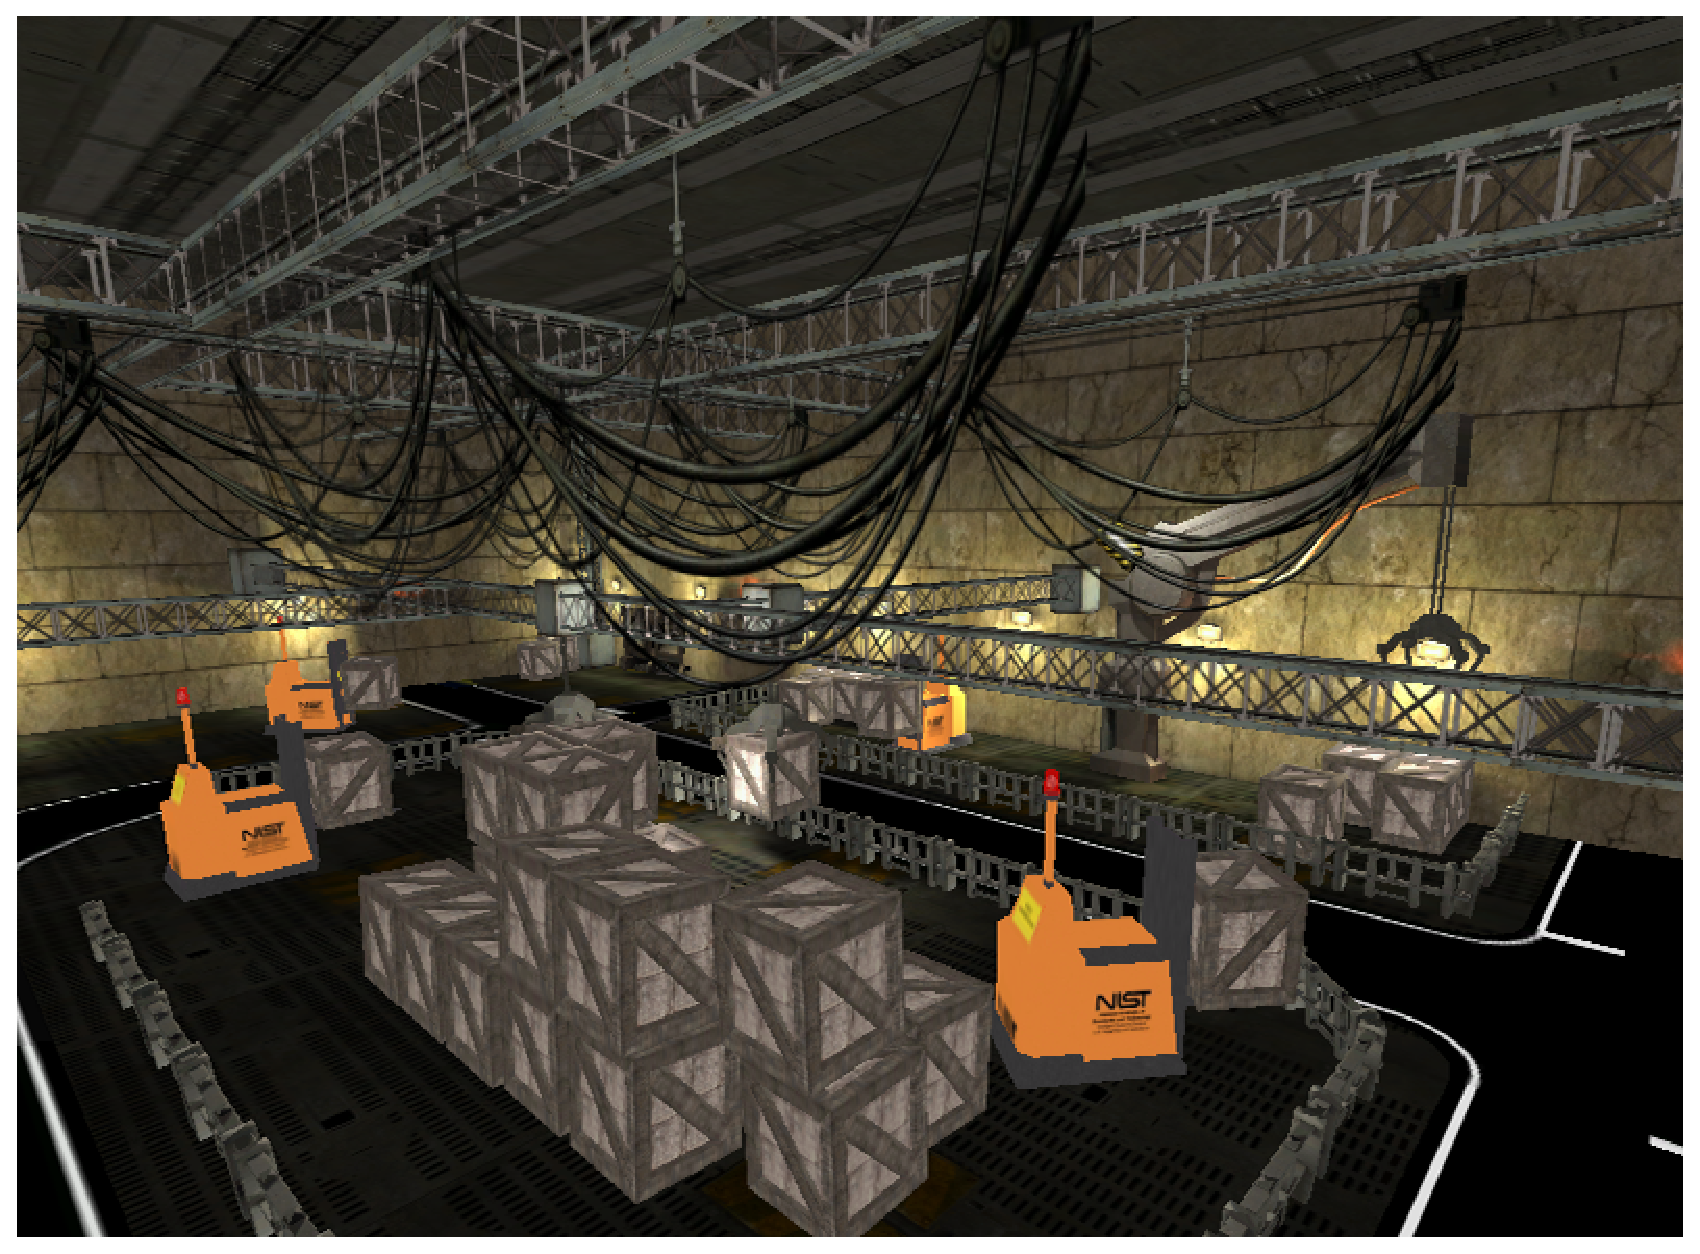
\psfig{file=Figures/Worlds/factory.eps,width=4cm}}%
\caption{Sample of 3D environments in USARSim.} \label{3D_World}
\end{figure}

USARSim was initially developed with a focus on wheeled robots, in
particular differential drive systems. Interest and wide community
support offer multiple robots, including underwater vehicles, legged
platforms, and humanoids. In USARSim, robots are based on the real
robots and are implemented by specific classes, thus making it
easier to develop new platforms that model custom designs. Three
base classes model different kinds of wheeled locomotion, namely
differential drives (Figure~\ref{Differential}), omnidirectional
vehicles (Figure~\ref{Omnidirectional}) and Ackerman steered
vehicles (Figures~\ref{Ackerman}).



All robots in USARSim have a chassis, multiple wheels, sensors and
effecters. The robots are configurable (specify types of
sensors/effecters for example). The properties of the robots can
also be configured, such as the battery life and the frequency of
data transmission.

\begin{figure}[t!]
\centering
\subfigure[ ATRV Jr.]{\label{Differential}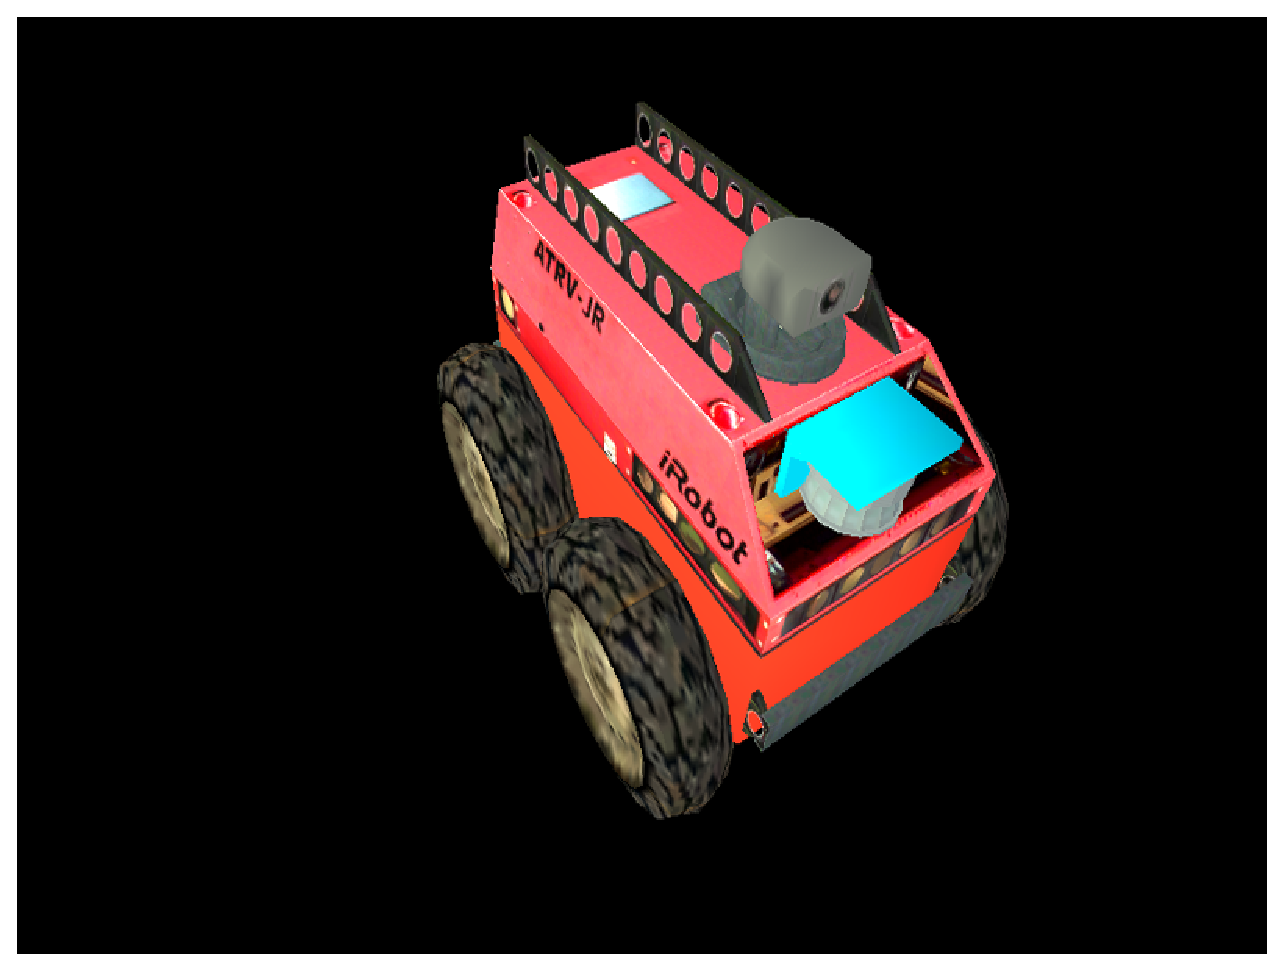
\psfig{file=Figures/Robots/ATRV-JR.eps,width=4cm}}\qquad
\subfigure[Passarola.]{\label{Omnidirectional}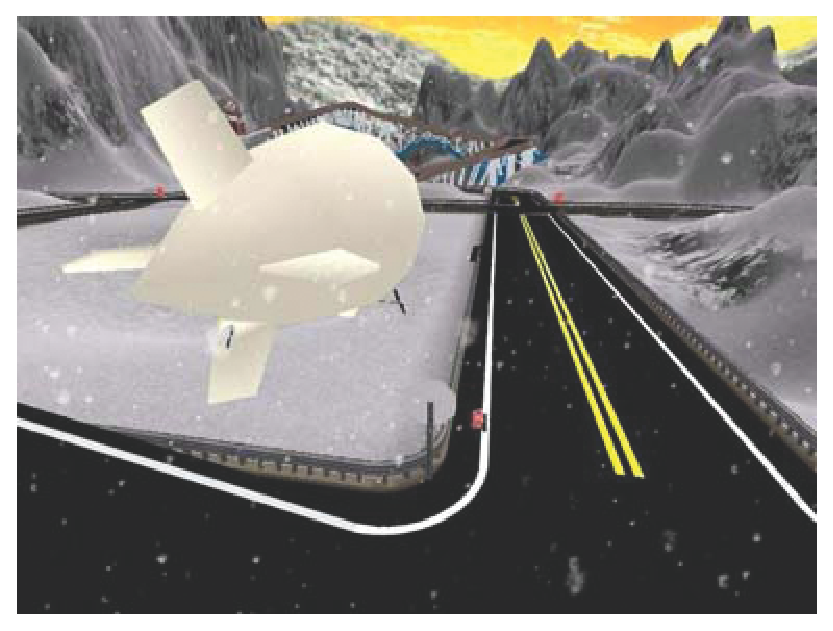
\psfig{file=Figures/Robots/passarola.eps,width=4cm}}\qquad
\subfigure[ NIST HMMWV.]{\label{Ackerman}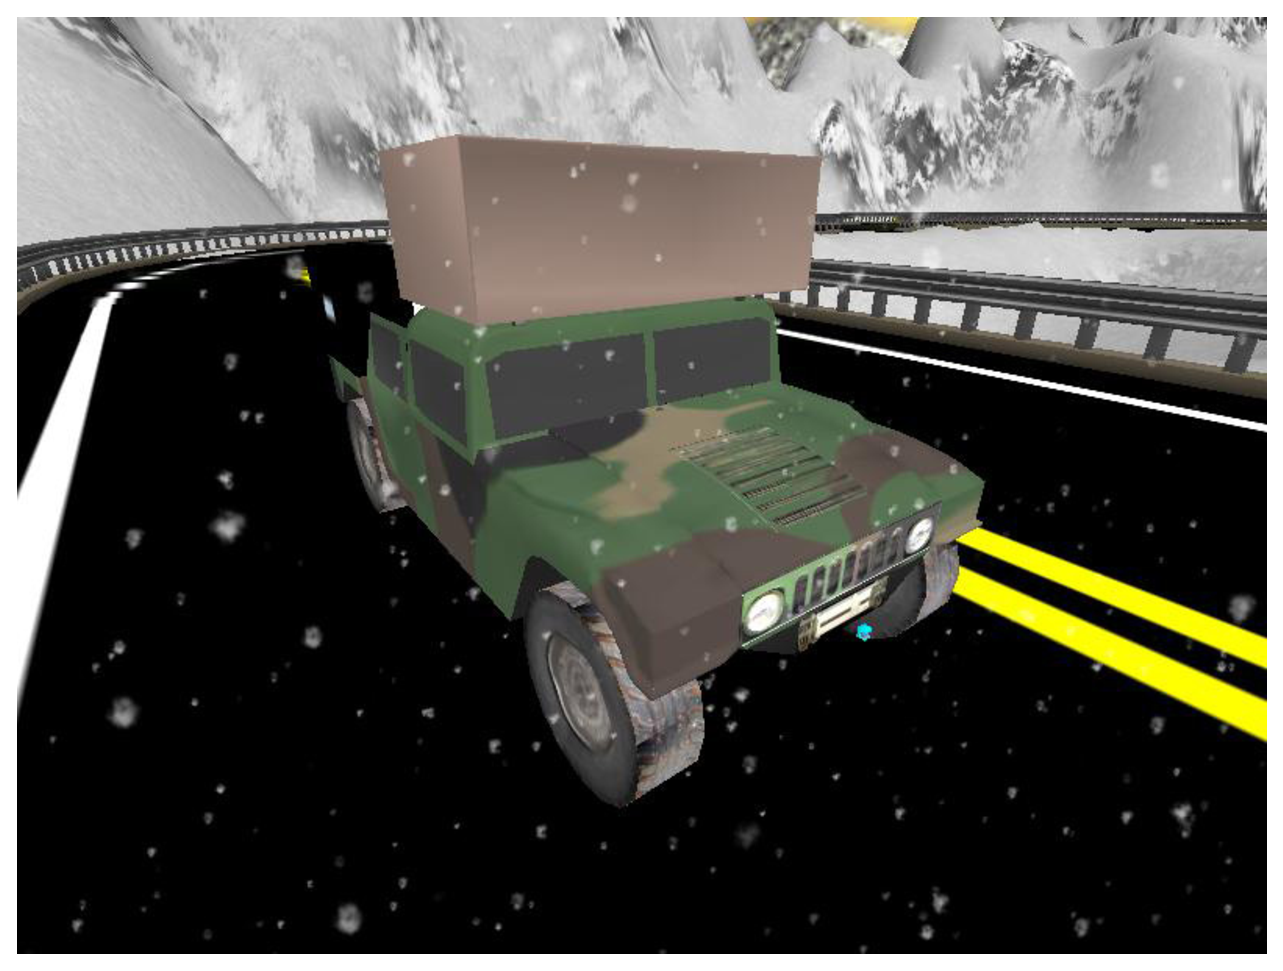
\psfig{file=Figures/Robots/hmmwv1.eps,width=4cm}}
\caption{Sample of vehicles in USARSim.}
\end{figure}


\subsection*{The ROS Framework}

ROS\footnote{http://www.ros.org/wiki/} is an open source framework designed to provide an abstraction layer to complex robotic hardware and software configurations. ROS delivers libraries and tools to help software developers create robot applications. ROS has been used in many robotic applications such as
Willow Garage\footnote{http://pr.willowgarage.com} Personal Robots Program~\cite{WYOBEK.ICRA.2008} and the Stanford University\footnote{http://stair.stanford.edu}
STAIR project~\cite{QUIGLEY.AAAI.2007}.


ROS possesses a large range of tools and services that both users and developers alike can benefit from. The philosophical goals of ROS include an advanced set of criteria and can be summarized as: peer-to-peer, tools-based, multi-lingual, thin, and free and open-source~\cite{QUIGLEY.ICRA.2009}. Furthermore, debugging at all levels of the software is made possible with the full source code of ROS being publicly available. Thus, the main developers of a project could benefit from the community and vice-versa.

\subsubsection*{Nomenclature}

The fundamental concepts of the ROS implementation are
nodes, messages, topics, and services. These terms will be used throughout the rest of the paper and are detailed below~\cite{QUIGLEY.ICRA.2009}.
\begin{itemize}
\item[-] Node: An executable unit which communicates with other nodes. ROS is
designed to be modular at a fine-grained scale: a system
is typically comprised of many nodes. In this context, the
term ``node" is interchangeable with ``software module". Nodes communicate with each other by passing messages.
\item[-] Message: A strictly typed data structure. Standard
primitive types (integer, floating point, boolean, \ldots) are
supported, as are arrays of primitive types and constants. A node sends a message by publishing it to a given topic.
\item[-] Topic: A communication channel between two or more
nodes. A node that is interested in a certain kind of data will subscribe
to the appropriate topic. There may be multiple concurrent
publishers and subscribers for a single topic, and a single
node may publish and/or subscribe to multiple topics.
\item[-] Service: A remote procedure call defined by a string name and a pair
of strictly typed messages: one for the request and one for
the response.
\item[-] Stack: Packages in ROS are organized into ROS stacks. Whereas the goal of packages is to create minimal collections of code for easy reuse, the goal of stacks is to simplify the process of code sharing. Stacks are the primary mechanism in ROS for distributing software. Each stack has an associated version and can declare dependencies on other stacks. These dependencies also declare a version number, which provides greater stability in development.
\end{itemize} 